\documentclass{beamer}

\usepackage[utf8]{inputenc}
\usepackage[absolute,overlay]{textpos}

\title{Model Checking World Domination}
\author{Jacob Errington \& Kevin Li}
\institute{McGill University}
\date{29 March 2017}

%%%%% PACKAGES

\usepackage{tikz}
\usepackage{textcomp}
\usepackage{amsmath,amssymb,amsthm}
\usepackage{listings}
\usepackage{graphicx}

%%%%% TIKZ

\usetikzlibrary{arrows,shapes,calc,graphs}

\tikzstyle{every picture}+=[remember picture]
\tikzset{
    ampersand replacement=\&,
    >=stealth',
    shorten >=1pt,
}

%%%%% THEOREMS

\theoremstyle{definition}
\newtheorem{defn}{Definition}

%%%%% LISTINGS

\lstset{basicstyle=\footnotesize\ttfamily}

%%%%% FONTS

\everymath{\displaystyle}
\usefonttheme{serif}

\setbeamercolor{framesource}{fg=gray}
\setbeamerfont{framesource}{size=\tiny}

%%%%% THEME

\usetheme{metropolis}

%%%%% COMMANDS 

\newcommand{\source}[1]{\begin{textblock*}{8cm}(0.5cm,8.6cm)
    \begin{beamercolorbox}[ht=0.5cm,left]{framesource}
        \usebeamerfont{framesource}\usebeamercolor[fg]{framesource} Source: {#1}
    \end{beamercolorbox}
\end{textblock*}}

\begin{document}

\frame{\titlepage}

\begin{frame}
    \frametitle{Robot apocalypse}

    \includegraphics[width=\textwidth]{nanobots.png}

    \pause

    \begin{itemize}
        \item
            If you're going to take over the world, \alert{do it right.}
    \end{itemize}
\end{frame}

\begin{frame}
    \frametitle{Philosophy of Swarm Robotics}
    \begin{itemize}
        \item
    "Achieve some desired, complex behavior using a collection of simple, individual agents."
    \end{itemize}
\end{frame}

% How swarm robotics and formal verification are connected
\begin{frame}
    \frametitle{Swarm Robotics - Formal Verification}

    \begin{itemize}
        \item Verification of swarm behavior (based on knowledge of individual design)
        \item \textbf{Optimization of swarm behavior}
    \end{itemize}
\end{frame}

% The results of real world actions are often uncertain. This motivates
% the usage of a probabilistic model to represent battles.
% We opt for the usage of discrete time Markov chains for simplicity
% and ease of construction. Our proposed model can be extended to
% continuous-time if necessary.
\begin{frame}
    \frametitle{DTMCs}
    \begin{defn}
        A \emph{discrete-time Markov Chain} (DTMC)
        is a tuple: $$ \mathcal{M} = (S, \mathbf{P}, \mathcal{d}_{init}, AP, L) $$
        \begin{itemize}
            \item $ S $ is the set of states,
            \item $ \mathbf{P} : S \times S \to [0, 1] $ is the transition probability function (matrix),
            \item $ \mathcal{d}_{init} : S \to [0, 1] $ is the initial distribution over states,
            \item AP, L as seen in class.
        \end{itemize}
    \end{defn}
\end{frame}

% Simple example of a DTMC.
% The point is to talk about probabilistic
% properties, like expectation.
\begin{frame}
    \frametitle{Example DTMC}
    \begin{center}
        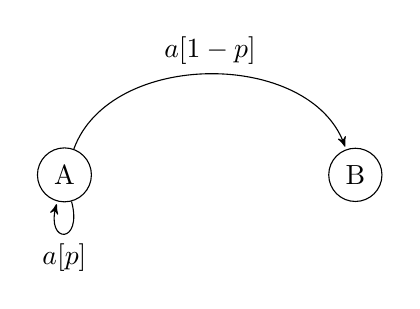
\begin{tikzpicture}
            \matrix[row sep=3cm, column sep=3cm]{
                \node[draw=black,circle] (A) {A} ; \&
                \node[draw=black,circle] (B) {B} ; \\
            } ;

            \graph[use existing nodes] {
                A ->[edge label={$a[p]$},loop below]
                A ->[edge label={$a[1-p]$},bend left=70]
                B ;
            } ;
        \end{tikzpicture}
    \end{center}
\end{frame}

\begin{frame}
    \frametitle{Property Specification in PCTL}

    \begin{itemize}
        \item Probabilistic extension of CTL.
        \item Additional semantics involving probability thresholds
            \begin{itemize}
                \item $ s \vdash \mathcal{P}_{\sim\lambda}(f_1 \text{ U } f_2) $
                \item $ s \vdash \mathcal{P}_{\sim\lambda}(\square f) $
                \item where $ \sim \in \{ >, <, \leq, \geq \} $
            \end{itemize}
        \item AP = $ \{ 1, \ldots, n \} $ describing the current number of
            messages in a queue.

            "The number of messages eventually reaches 3 with probability of at least 0.5"
            $ \iff \mathcal{P}_{\geq 0.5}(true \text{ U } 3) $
    \end{itemize}
\end{frame}

% Now introduce an example of a PTS that would
% be used in swarm robotics: the foraging
% swarm example.
% 
% Each edge is annotated with a probability.
% 
% This transition system demonstrates the behavior
% of a single robot. To get the behavior of the swarm,
% we could perform parallel composition on a ton of such
% transition systems, but the state-space would grow
% exponentially. Thus, this problem is treated by adding
% a count on each state of the number of robots that are in that
% state. Updates to those counts happen corresponding to the probability
% of going to other states.
%
% The purpose of this simulation was to measure the
% "total energy" levels in the population of foraging robots,
% which decrease whenever an action is taken by a robot,
% and increase whenever a robot deposits food at home.
% 
% Interesting properties can be verified, such as
% "what is the probability that energy levels will
% always be above zero?"
\begin{frame}
    \frametitle{DTMC Model for Foraging Swarm}

    \begin{center}
        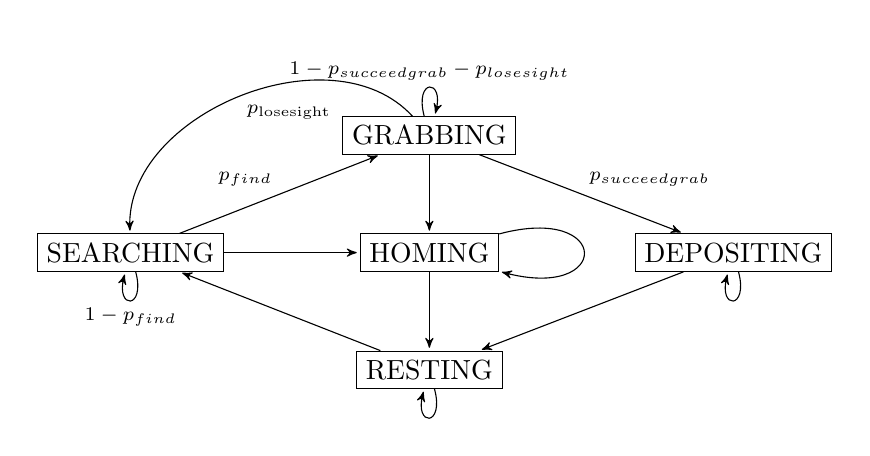
\begin{tikzpicture}
            \matrix[row sep=1cm,column sep=1.5cm]{
                \& \node[draw=black,rectangle] (grab) {GRABBING} ; \& \\
                \node[draw=black,rectangle] (search) {SEARCHING} ; \&
                \node[draw=black,rectangle] (home) {HOMING} ; \&
                \node[draw=black,rectangle] (deposit) {DEPOSITING} ; \\
                \& \node[draw=black,rectangle] (rest) {RESTING} ; \& \\
            } ;

            \scriptsize

            \graph[use existing nodes] {
                grab ->[loop above,edge label={$1 - p_{succeedgrab} - p_{losesight}$}]
                grab ->[bend right=70,edge label={$p_{\text{losesight}}$}] search;
                grab ->[edge label={$p_{succeedgrab}$}] deposit;
                grab -> home;

                search ->[edge label={$p_{find}$}] grab;
                search -> home;
                search ->[edge label={$1-p_{find}$},loop below] search;

                home ->[loop right] home;
                home -> rest;

                deposit ->[loop below]
                deposit -> rest;

                rest ->[loop below]
                rest -> search;
            } ;
        \end{tikzpicture}
    \end{center}
    \source{Konur, Savas, Clare Dixon, and Michael Fisher. \textit{"Formal verification of probabilistic swarm behaviours."} International Conference on Swarm Intelligence. Springer Berlin Heidelberg, 2010.}
\end{frame}

\begin{frame}
    \frametitle{Limitations to Studying Foraging}

    \begin{itemize}
        \item No notion of the benefit of cooperation
        \item Robots act entirely independent of one another
        \item Does not take advantage of aggregation/disaggregation ability
    \end{itemize}
\end{frame}

\begin{frame}
    \frametitle{Problem - Swarm Task Allocation}

    \begin{itemize}
        \item How to optimally allocate robots among similar
            \textbf{concurrent, probabilistic tasks} of \textbf{heterogeneous difficulty}?
    \end{itemize}
\end{frame}

\begin{frame}
    \frametitle{Traits of Distributable Probabilistic Tasks (DPTs)}
    \begin{itemize}
        \item Probabilistic completion
        \item Cooperative
        \item Concurrent
        \item Heterogeneous difficulty
        \item Redistributable
    \end{itemize}
\end{frame}

\begin{frame}
    \frametitle{Examples of DPTs}

    \begin{itemize}
        \item Battle scenario w/ multiple enemies
        \item Cryptocurrency mining
        \item DDOS attack planning
        \item Search and rescue
        \item Grannies baking for their church bakesale
    \end{itemize}
\end{frame}

% Must mention that the key is the probabilities for winning
% in a round of battle are different in each TS.
% They are functions of c, n, and l.
% The probabilities are represented in the following way.
\begin{frame}
    \frametitle{Battle Model}

    \begin{itemize}
        \item
            $N$ bots, $M \subset \mathbb{N} \times \mathbb{N} $ finite targets.
            Each element in $ M $ is a pair, where the first element is
            the ID of the enemy, and the second is the difficulty level.

            All IDs must be unique.
            %
        \item
            Targets become neutralized probabilistically.
            %
        \item
            Agents can cooperate to defeat targets w/ higher probability.
            %
        \item
            Upon target neutralization, robots may redistribute over
            remaining battles.
    \end{itemize}

    \begin{center}
        \begin{tikzpicture}
            \matrix[row sep=1cm, column sep=4cm]{
                \node (A) {$A_i$} ; \&
                \node (E) {$E_i$} ; \&
                \node (K) {$K_i$} ; \\
            } ;

            \graph[use existing nodes] {
                A ->[edge label={init}]
                E ->[edge label={$atk[p_i]$},loop above]
                E ->[edge label={$atk[1-p_i]$}]
                K;
            } ;
        \end{tikzpicture}

        Battle $ i $
    \end{center}
\end{frame}

% We may represent these attacking probabilities in any number of ways,
% but we have chosen:

% Because the prob is a function of the level, this encodes the heterogeneity
% of difficulty.

% The lambda paramter (1 / cn) encodes the idea that cooperation improves
% performance, and so does this notion of "robot efficiency".

% Keep in mind that our goal was to optimally redistribute!
\begin{frame}
    \frametitle{Probabilistic Attacking}

    Suppose $n$ bots are allocated to enemy $i$, of level $l$.
    Bots have an efficiency rating $c$.

    \begin{center}
        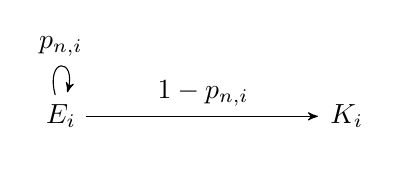
\begin{tikzpicture}
            \matrix[row sep=4cm, column sep=3cm]{
                \node (E) {$E_i$} ; \&
                \node (K) {$K_i$} ; \\
            } ;

            \graph[use existing nodes] {
                E ->[edge label={$p_{n,i}$},loop above]
                E ->[edge label={$1-p_{n,i}$}]
                K ;
            } ;
        \end{tikzpicture}
    \end{center}

    \pause

    \begin{itemize}
        \item
            Probability of defeating the enemy grows as $n$ increases.

            \begin{equation*}
                p_{n,i} = e^{-\frac{l}{cn}}
            \end{equation*}
            %
        \item
            The number $n_i$ of bots attacking this enemy changes as other
            enemies are defeated and redistribution occurs.
    \end{itemize}
\end{frame}

% What is a good rule?
\begin{frame}
    \frametitle{Optimal Redistribution Policy}
    Battle $ i $ has ended.

    Let set of states $ \mathcal{F} = \{ j \text{ s.t. } j \neq i \wedge \text{Battle } j \text{ not ended} \} $.

    Goal : redistribute bots of $ i $ among all $ j \in \mathcal{F} $.

    $ l_j $ : enemy $ j $'s level

    $ n_j $ : number of robots currently attacking enemy $ j $.

    \begin{itemize}
        \item<1-> Naive weighted average of levels
        \item<2-> Adjusted weighted average
        \item<3-> Adjusted weight average w/ function
    \end{itemize}
    \begin{equation*}
        \only<1>{\frac{l_j}{\displaystyle\sum_{k \in \mathcal{F}}{l_k}}}
        \only<2>{\frac{\frac{l_i}{cn_i}}{\displaystyle\sum_{k \in \mathcal{F}}{\frac{l_k}{cn_k}}}}
        \only<3>{\frac{g(\frac{l_i}{cn_i})}{\displaystyle\sum_{k \in \mathcal{F}}{g(\frac{l_k}{cn_k})}}}
    \end{equation*}
\end{frame}

% Further model definition
\begin{frame}
    \frametitle{Casualties}

    Probabilistically lose robots if a round of combat is unsuccessful.
    
    Parameter $ b \in [0, 1] $ governs this.
\end{frame}

\begin{frame}
    \frametitle{Implementation}

    \begin{itemize}
        \item PRISM code generation in Haskell
        \item Cloud computing for model construction
            \begin{itemize}
                \item
            \end{itemize}
    \end{itemize}
\end{frame}

\end{document}
